%% Author: Leighton Pritchard
%% Copyright: James Hutton Institute
%% 2016-05-23: Slides for teaching at EMBL/EBI, 23rd May 2016
%% This presentation was an invited lecture on Pathogen Genome Data as
%% part of the Bioinformatics of Plants and Plant Pathogens

%% UNCOMMENT FOR SLIDES
\documentclass[table]{beamer}
\mode<presentation>

%% UNCOMMENT FOR HANDOUTS
%\input{sections/preamble_handouts}
%% GENERIC STYLE SETTINGS BELOW
\usetheme{default}
\usepackage{listings}
\usepackage{multirow}
\usepackage{xcolor}
\usepackage{hyperref}
%\usepackage[multiple]{footmisc}

\usebackgroundtemplate{

\includegraphics[width=\paperwidth,height=\paperheight]{images/hutton_background}
}
%% PRESENTATION CONFIGURATION PARAMETERS %%%%%%%%%%%%%%%%%%%%%%%%%%%%%%%%%%%%%%%
%\titlebackgroundfile{images/hutton_title}
%\framebackgroundfile{images/hutton_background}
\definecolor{hutton_green}{HTML}{78A22F}
\definecolor{hutton_purple}{HTML}{872175}
\definecolor{hutton_blue}{HTML}{569BBE}
\definecolor{olive}{rgb}{0.3, 0.4, .1}
\definecolor{fore}{RGB}{249,242,215}
\definecolor{back}{RGB}{51,51,51}
\definecolor{title}{RGB}{255,0,90}
\definecolor{dgreen}{rgb}{0.,0.6,0.}
\definecolor{gold}{rgb}{1.,0.84,0.}
\definecolor{JungleGreen}{cmyk}{0.99,0,0.52,0}
\definecolor{BlueGreen}{cmyk}{0.85,0,0.33,0}
\definecolor{RawSienna}{cmyk}{0,0.72,1,0.45}
\definecolor{Magenta}{cmyk}{0,1,0,0}
\usefonttheme{structurebold}
\setbeamercolor{alerted text}{fg=orange}
\setbeamercolor{background canvas}{bg=white}
\setbeamercolor{block title}{bg=hutton_purple}
\setbeamercolor{frametitle}{fg=hutton_purple}
\setbeamercolor{title}{fg=black}
\setbeamercolor{titlelike}{fg=hutton_green}
\setbeamercolor{author}{fg=hutton_purple}
\setbeamercolor{author in head/foot}{fg=white}
\setbeamercolor{title in head/foot}{fg=white}
\setbeamercolor{section in head/foot}{fg=hutton_purple}
\setbeamercolor{normal text}{fg=black}
\setbeamercolor{frametitle}{fg=hutton_purple}
\setbeamerfont{author}{size=\footnotesize}
\setbeamerfont{institute}{size=\tiny}
\setbeamerfont{date}{size=\footnotesize}
\setbeamercolor{section in toc shaded}{fg=hutton_purple}
\setbeamercolor{section in toc}{fg=hutton_purple}
\setbeamercolor{subsection in toc shaded}{fg=hutton_purple}
\setbeamercolor{subsection in toc}{fg=hutton_purple}
\setbeamertemplate{itemize item}[circle]
\setbeamertemplate{itemize subitem}[circle]
\setbeamertemplate{itemize subsubitem}[circle]
\setbeamertemplate{itemize subsubsubitem}[circle]
\setbeamercolor{itemize item}{fg=hutton_purple}
\setbeamercolor{itemize subitem}{fg=hutton_purple}
\setbeamercolor{itemize subsubitem}{fg=hutton_purple}
\setbeamercolor{itemize subsubsubitem}{fg=hutton_purple}
\setbeamercolor{enumerate item}{fg=hutton_purple}
\setbeamercolor{enumerate subitem}{fg=hutton_purple}
\setbeamercolor{enumerate subsubitem}{fg=hutton_purple}
\setbeamercolor{enumerate subsubsubitem}{fg=hutton_purple}
% ALERTS AND BLOCKS
\setbeamercolor{alerted text}{fg=hutton_green}
\setbeamerfont{alerted text}{series=\bfseries}
\setbeamercolor{block title}{use=structure,fg=white,bg=structure.fg!75!black}
\setbeamercolor{block title alerted}{use=alerted text,fg=white,bg=alerted text.fg!75!black}
\setbeamercolor{block title example}{use=example text,fg=white,bg=example text.fg!75!black}
\setbeamercolor{block body}{parent=normal text,use=block title,bg=block title.bg!10!bg}
\setbeamercolor{block body alerted}{parent=normal text,use=block title alerted,bg=block title alerted.bg!10!bg}
\setbeamercolor{block body example}{parent=normal text,use=block title example,bg=block title example.bg!10!bg}
% This command makes sure that acrobat reader doesn't change the colours of the slide
% when there are figures with transparencies.
\pdfpageattr {/Group << /S /Transparency /I true /CS /DeviceRGB>>}

%Disables discrete bottom navigation bar
\beamertemplatenavigationsymbolsempty

% Modify the slide titles to avoid the corner images,
\setbeamertemplate{frametitle}
{
\vspace{0.05\textheight}
\noindent\quad\begin{minipage}[t][0.12\textheight][t]{0.85\textwidth}
\insertframetitle\par
\end{minipage}
}

% Modify title page to avoid the big logo on right
\setbeamertemplate{title page}{
    \begin{picture}(0,0)
            %This ends up on top of the default background image, rather than replacing it:
            \put(-30,-165){%
                
\includegraphics[width=\paperwidth,height=\paperheight]{images/hutton_title}
            }
            \put(0,-75){%
                \begin{minipage}[b][0.4\textheight][t]{0.75\textwidth}
                    \usebeamerfont{title}\usebeamercolor[fg]{title}{\inserttitle\par}
                    \usebeamerfont{subtitle}\usebeamercolor[fg]{subtitle}{\insertsubtitle\par}
                \end{minipage}
            }
            \put(0,-125){%
                \begin{minipage}[b][0.1\textheight][t]{\textwidth}
                    \usebeamerfont{author}\usebeamercolor[fg]{author}{\insertauthor\par}
                    \usebeamerfont{institute}\usebeamercolor[fg]{institute}{\insertinstitute\par}
                \end{minipage}
            }
    \end{picture}
}

% Make \verbatim environment tiny font
\makeatletter
\def\verbatim{\tiny\@verbatim \frenchspacing\@vobeyspaces \@xverbatim}
\makeatother

% Inner Theme for Blocks
\useinnertheme{rectangles}

%%%%%%%%%%%%%%%%%%%%%%%%%%%%%%%%%%%%%%%%%%%%%%%%%%%%%%%%%%%%%%%%%%%%%%%%%%%%%%%%

% LISTINGS SETTING
% Settings for code listings in lstlistings

\definecolor{hutton_lightgreen}{HTML}{C8F27F}

\lstset{ %
  backgroundcolor=\color{hutton_lightgreen},   % choose the background color; you must add \usepackage{color} or \usepackage{xcolor}
  basicstyle=\tiny\ttfamily,        % the size of the fonts that are used for the code
  breakatwhitespace=false,         % sets if automatic breaks should only happen at whitespace
  breaklines=true,                 % sets automatic line breaking
  captionpos=b,                    % sets the caption-position to bottom
  commentstyle=\color{red},    % comment style
  deletekeywords={...},            % if you want to delete keywords from the given language
  escapeinside={\%*}{*)},          % if you want to add LaTeX within your code
  extendedchars=true,              % lets you use non-ASCII characters; for 8-bits encodings only, does not work with UTF-8
  frame=single,                    % adds a frame around the code
  keepspaces=true,                 % keeps spaces in text, useful for keeping indentation of code (possibly needs columns=flexible)
  keywordstyle=\color{blue},       % keyword style
%  language=Octave,                 % the language of the code
  morekeywords={*,...},            % if you want to add more keywords to the set
  numbers=left,                    % where to put the line-numbers; possible values are (none, left, right)
  numbersep=5pt,                   % how far the line-numbers are from the code
  numberstyle=\tiny\color{gray}, % the style that is used for the line-numbers
  rulecolor=\color{black},         % if not set, the frame-color may be changed on line-breaks within not-black text (e.g. comments (green here))
  showspaces=false,                % show spaces everywhere adding particular underscores; it overrides 'showstringspaces'
  showstringspaces=false,          % underline spaces within strings only
  showtabs=false,                  % show tabs within strings adding particular underscores
  stepnumber=1,                    % the step between two line-numbers. If it's 1, each line will be numbered
  stringstyle=\color{violet},     % string literal style
  tabsize=4,                       % sets default tabsize to 2 spaces
  title=\lstname                   % show the filename of files included with \lstinputlisting; also try caption instead of title
}


%%%
% TITLE PREAMBLE
\title[Pathogen Genome Data] % (optional, only for long titles)
{Pathogen Genome Data \\
{\small EMBL-EBI Bioinformatics of Plants and \\ Plant Pathogens 23$^{rd}$ May 2016}}
%\subtitle{}
\author[Leighton Pritchard] % (optional, for multiple authors)
{Leighton~Pritchard$^{1,2,3}$}
\institute[The James Hutton Institute] % (optional)
{
  $^{1}$Information and Computational Sciences,\\
  $^{2}$Centre for Human and Animal Pathogens in the Environment,\\
  $^{3}$Dundee Effector Consortium,\\
  The James Hutton Institute, Invergowrie, Dundee, Scotland, DD2 5DA
}
\date[23rd May 2016] % (optional)
{23rd May 2016}
\subject{Bioinformatics, Genomics, Plant Pathogens, Plants, Microbiology, Microbes, Comparative Genomics, Visualisation}

%%%
% TOC
% Show table of contents, with current section highlighted,
% at the start of each section

%\AtBeginSection[]
%{
%  \begin{frame}
%    \frametitle{Table of Contents}
%    \tableofcontents[currentsection] %,hideallsubsections]
%  \end{frame}
%}

\AtBeginSubsection[]
{
  \begin{frame}
    \frametitle{Table of Contents}
    \tableofcontents[currentsection,currentsubsection] %,hideallsubsections]
  \end{frame}
}

%%%
% START DOCUMENT
\begin{document}

\frame[plain]{\titlepage}

%% use.tex
%% Author: Leighton Pritchard
%% Copyright: James Hutton Institute
%% These slides describe the acceptable use policy for these slides and
%% materials

%
\begin{frame}
  \frametitle{Acceptable Use Policy}
  Recording of this talk, taking photos, discussing the content using \\
  email, Twitter, blogs, etc. is permitted (and encouraged), \\
  providing distraction to others is minimised. \\[0.5cm]
  These slides will be made available on SlideShare. \\[0.5cm]
  \textbf{These slides, and supporting material including exercises, are available at \href{https://github.com/widdowquinn/Teaching-EMBL-Plant-Path-Genomics}{https://github.com/widdowquinn/Teaching-EMBL-Plant-Path-Genomics}}
\end{frame}

%%%
%% SECTION: Introduction
\section{Introduction}

%% SUBSECTION
%% Pathogen Genome Data
\subsection{Pathogen Genome Data}
%% pathogen_genome_data.tex
%% Copyright: James Hutton Institute 2016
%% Author: Leighton Pritchard
%% Pathogen Genome Data

%
\begin{frame}
  \frametitle{Introduction}
    \begin{alertblock}{What can pathogen genome data do for you?}
        A combination of genomic data, and comparative and evolutionary biology, 
        can address questions of pathogen evolution, adaptation and lifestyle.
    \end{alertblock}
\end{frame}


\begin{frame}
  \frametitle{}

  \begin{block}{Block Title}
    Test Block
  \end{block}
\end{frame}

%%%
%% SECTION: Public Data Sources
\section{Public Data Sources}

%% SUBSECTION
%% Online Resources
\subsection{Online Resources}
%% public_data_sources.tex
%% Copyright: James Hutton Institute 2016
%% Author: Leighton Pritchard
%% Public Data Sources

% NCBI
\begin{frame}
  \frametitle{NCBI \hfill 
\includegraphics[height=0.1\textheight,valign=t]{images/NCBI}}
    \begin{alertblock}{\href{http://www.ncbi.nlm.nih.gov/}{http://www.ncbi.nlm.nih.gov/}}
      Repository of record for pathogen (and other) genome data
    \end{alertblock}
    \begin{itemize}
      \item Example: \textcolor{hutton_purple}{\href{http://www.ncbi.nlm.nih.gov/genome/490}{\textit{Ralstonia solanacearum}}}
        \begin{itemize}
          \item Browser interface
          \item FTP repositories of genome data \\
            - \textcolor{hutton_purple}{\href{http://ftp.ncbi.nlm.nih.gov/genomes/refseq/bacteria/Ralstonia_solanacearum/latest_assembly_versions/}{RefSeq}} \\
            - \textcolor{hutton_purple}{\href{http://ftp.ncbi.nlm.nih.gov/genomes/genbank/bacteria/Ralstonia_solanacearum/latest_assembly_versions/}{GenBank}}
        \end{itemize}
    \end{itemize}
    \begin{center}
      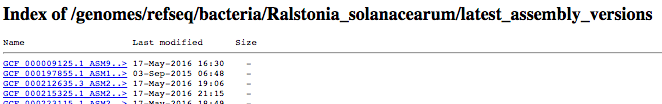
\includegraphics[width=0.75\textwidth]{images/refseq_list} \\ 
      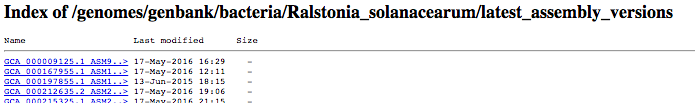
\includegraphics[width=0.75\textwidth]{images/genbank_list}      
    \end{center}    
\end{frame}

% GENBANK VS REFSEQ
\begin{frame}
  \frametitle{GenBank \textit{vs} RefSeq}
    \begin{alertblock}{\href{http://www.ncbi.nlm.nih.gov/genbank/}{GenBank}}
      \begin{itemize}
        \item part of \textcolor{hutton_purple}{\href{http://www.insdc.org/}{International Nucleotide Sequence Database Collaboration (INSDC)}}: EMBL/NCBI/DDBJ
        \item records 'owned' by submitter
        \item may include redundant information
      \end{itemize}
    \end{alertblock}
    \begin{block}{\href{http://www.ncbi.nlm.nih.gov/refseq/about}{RefSeq}}
      \begin{itemize}
        \item not part of INSDC
        \item records derived from GenBank, 'owned' by NCBI
        \item stable non-redundant foundation for functional and diversity studies
      \end{itemize}
    \end{block}
\end{frame}

% ENSEMBL
\begin{frame}
  \frametitle{Ensembl \hfill 
\includegraphics[height=0.1\textheight,valign=t]{images/ensembl_metazoa_logo}}
    \begin{alertblock}{\href{http://www.ensembl.org}{http://www.ensembl.org}}
      Automated annotation on selected genomes
    \end{alertblock}
    \begin{itemize}
      \item \textbf{Specialised sub-collections}
      \begin{itemize}
        \item Ensembl Protists: \textcolor{hutton_purple}{\href{http://protists.ensembl.org/}{http://protists.ensembl.org/}}
        \item Ensembl Bacteria: \textcolor{hutton_purple}{\href{http://bacteria.ensembl.org/}{http://bacteria.ensembl.org/}}
        \item Ensembl Fungi: \textcolor{hutton_purple}{\href{http://fungi.ensembl.org/}{http://fungi.ensembl.org/}}
      \end{itemize}
      \item \textbf{Downloadable resource}
      \begin{itemize}
        \item e.g. \textcolor{hutton_purple}{\href{http://ftp.ensemblgenomes.org/pub/protists/}{ftp://ftp.ensemblgenomes.org/pub/protists/}}
      \end{itemize}
      \item \textbf{Ready-made comparative genomics!}      
      \begin{itemize}
        \item \textcolor{hutton_purple}{\href{http://protists.ensembl.org/Phytophthora_infestans/Location/Compara_Alignments/Image?align=119329;db=core;r=supercont1.34:559462-573700}{\textit{Phytophthora} genomics alignments (Avr3a)}}
        \item \textcolor{hutton_purple}{\href{http://protists.ensembl.org/Phytophthora_infestans/Gene/Compara_Tree/pan_compara?db=core;g=PITG_14371;r=supercont1.34:559462-573700;t=PITG_14371T0}{Gene trees (Avr3a)}}
      \end{itemize}
    \end{itemize}
\end{frame}

% OTHER SOURCES
\begin{frame}
  \frametitle{Other Sources}
    \begin{itemize}
      \item \textbf{Sequencing centres, e.g.}
      \begin{itemize}
        \item \textcolor{hutton_purple}{\href{http://genome.jgi.doe.gov/}{JGI Genome Portals}}
        \item Ensembl Bacteria: \textcolor{hutton_purple}{\href{https://www.broadinstitute.org/}{Broad Institute}} - now retiring their online resources
      \end{itemize}
      \item \textbf{Specialist databases, e.g.}
      \begin{itemize}
        \item \textcolor{hutton_purple}{\href{http://fungidb.org/fungidb/}{FungiDB}} - fungi and oomycetes
        \item \textcolor{hutton_purple}{\href{http://cpgr.plantbiology.msu.edu/}{CPGR}} - fungi and oomycetes (not recently updated)
      \end{itemize}
      \item \textbf{Your friendly local sequencing centre!}      
      \begin{itemize}
        \item \textcolor{hutton_purple}{\href{http://asperasoft.com/}{Aspera}} is commonly used to connect to your private data
      \end{itemize}
    \end{itemize}
\end{frame}

% OPTIONAL WORKSHEET
\begin{frame}
  \frametitle{Optional Worksheet}
  \begin{alertblock}{\url{worksheets/01-downloading_data_biopython.ipynb}}
    Downloading genome data from NCBI with Biopython
  \end{alertblock}
  \begin{itemize}
    \item \textcolor{hutton_purple}{\href{http://mybinder.org/repo/widdowquinn/Teaching-EMBL-Plant-Path-Genomics}{MyBinder link}}
  \end{itemize}
\end{frame}


%%%
%% SECTION: Comparative Genomics
\section{Comparative Genomics}

%% SUBSECTION
%% Why Comparative Genomics?
\subsection{Why Comparative Genomics?}
%% why_comparative_genomics.tex
%% Copyright: James Hutton Institute 2016
%% Author: Leighton Pritchard
%% Why Comparative Genomics?

% WHY COMPARATIVE GENOMICS
\begin{frame}
  \frametitle{Why comparative genomics?}
    \begin{columns}[c] 
      \column{.6\textwidth} 
        \begin{itemize}
         \item \textcolor{hutton_green}{Transfer functional information from model systems (\textit{E. coli}, \textit{A. thaliana}, \textit{D. melanogaster}) to non-model systems}        
         \item \textcolor{hutton_blue}{Genome similarity $\propto$ phenotype? (\textit{functional genomics}): virulence and host range}         
         \item \textcolor{RawSienna}{Genome similarity $\propto$ relatedness? (\textit{phylogenomics}): record of evolutionary processes and constraints}
        \end{itemize}
      \column{.4\textwidth}
        
\includegraphics[width=\textwidth]{images/darwin_tree}
    \end{columns}  
\end{frame}

% WHY COMPARATIVE GENOMICS
\begin{frame}
  \frametitle{Genomes aren't everything$\ldots$}
    \begin{columns}[c] 
      \column{.6\textwidth} 
        \begin{alertblock}{Context}
          \begin{itemize}
            \item epigenetics
            \item tissue differentiation/differential expression
            \item mesoscale systems, etc.
          \end{itemize}
        \end{alertblock}
        \begin{block}{Phenotypic plasticity, responses to}         
          \begin{itemize}
            \item temperature
            \item stress
            \item community, etc.
          \end{itemize}
        \end{block}
        \textcolor{red}{$\ldots$and therefore systems biology$\ldots$}
      \column{.4\textwidth}
        
\includegraphics[width=\textwidth]{images/darwin_tree}
    \end{columns}  
\end{frame}

% LEVELS OF COMPARISON
\begin{frame}
  \frametitle{Levels of comparison}
    \begin{alertblock}{Bulk Properties}
      \begin{itemize}
        \item \textcolor{hutton_green}{e.g. $k$-mer spectra} (\textcolor{hutton_purple}{\href{https://github.com/marbl/Mash}{MaSH}}, \textcolor{hutton_purple}{\href{https://github.com/dkoslicki/MetaPalette}{MetaPalette}}, etc.)
      \end{itemize}
    \end{alertblock}
    \begin{block}{Whole Genome Sequence}
      \begin{itemize}
        \item \textcolor{hutton_blue}{sequence similarity} (\textcolor{hutton_purple}{\href{https://blast.ncbi.nlm.nih.gov/Blast.cgi?PAGE_TYPE=BlastDocs&DOC_TYPE=Download}{BLAST}}, \textcolor{hutton_purple}{\href{https://genome.ucsc.edu/FAQ/FAQblat.html}{BLAT}}, \textcolor{hutton_purple}{\href{http://mummer.sourceforge.net/}{MUMmer}}, etc.)
        \item \textcolor{hutton_blue}{structure and organisation} (\textcolor{hutton_purple}{\href{http://darlinglab.org/mauve/mauve.html}{Mauve}}, \textcolor{hutton_purple}{\href{http://www.sanger.ac.uk/science/tools/artemis-comparison-tool-act}{ACT}}, etc.)
      \end{itemize}
    \end{block}
    \begin{alertblock}{Genome Features/Functional Components}
      \begin{itemize}
        \item \textcolor{RawSienna}{numbers and types of features: genes, ncRNA, regulatory elements, etc.}
        \item \textcolor{RawSienna}{organisation of features: synteny, operons, regulons, etc.}
        \item \textcolor{RawSienna}{functional complement} (\textcolor{hutton_purple}{\href{http://www.genome.jp/kegg/}{KEGG}}, etc.)
      \end{itemize}
    \end{alertblock}
\end{frame}



% SECTION: Genome Comparisons
\section{Genome Comparisons}

%% SUBSECTION
%% Whole Genome Comparisons
\subsection{Whole Genome Comparisons}
%% whole_genome_comparisons.tex
%% Author: Leighton Pritchard
%% Copyright: James Hutton Institute 2016
%% Whole genome comparisons

% WHOLE GENOME COMPARISON
\begin{frame}
  \frametitle{Whole genome comparisons}
    \begin{alertblock}{Whole genome comparison}
      Comparisons of one complete or draft genome with another \\
      ($\ldots$or many others)
    \end{alertblock}
  Minimum requirement: \textbf{two genomes} \\
  \begin{itemize}
    \item \textcolor{hutton_green}{Reference Genome}
    \item \textcolor{hutton_blue}{Comparator Genome}
  \end{itemize}
  The experiment produces a comparative result \textcolor{hutton_purple}{\textit{that is dependent on the choice of genomes}}.    
\end{frame}

% PAIRWISE GENOME ALIGNMENT
\begin{frame}
  \frametitle{Pairwise genome alignments}
  \textcolor{olive}{Pairwise comparisons produce alignments of similar regions.}
  \begin{center}
    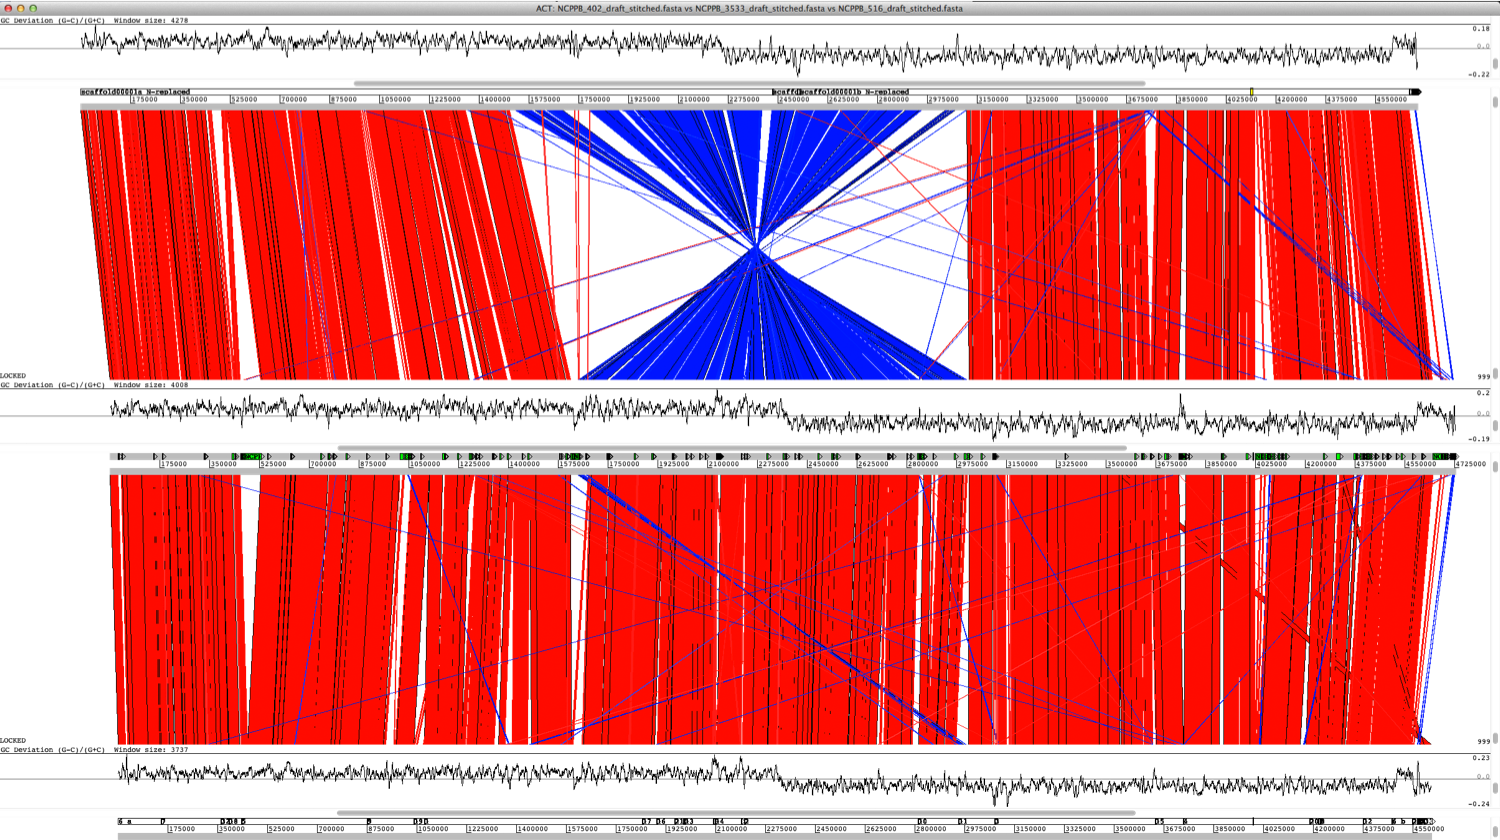
\includegraphics[width=\textwidth]{images/pairwise_genome_alignment}
  \end{center}  
\end{frame}

% SYNTENY AND COLLINEARITY
\begin{frame}
  \frametitle{Synteny and Collinearity}
  \textcolor{olive}{Genome rearrangements may occur post-species divergence} \\
  Sequence similarity, and order of similar regions, may be conserved
  \begin{center}
    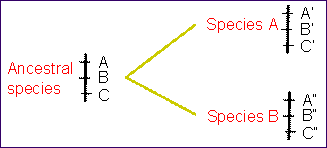
\includegraphics[width=0.5\textwidth]{images/collinear}    
    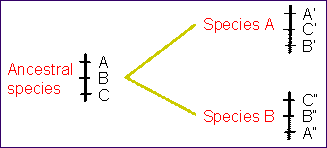
\includegraphics[width=0.5\textwidth]{images/synteny}
  \end{center}    
  \begin{itemize}
    \item \textcolor{hutton_blue}{\textit{collinear}} conserved elements lie in the same linear sequence
    \item \textcolor{hutton_purple}{\textit{syntenous} (or \textit{syntenic})} elements:
    \begin{itemize}
      \item (\textit{orig.}) lie on the same chromosome
      \item (\textit{mod.}) are collinear
    \end{itemize}
  \end{itemize}
  \textcolor{hutton_green}{Evolutionary constraint} (e.g. indicated by synteny) may indicate \textcolor{hutton_green}{functional constraint} (and help determine \textit{orthology})
\end{frame}

% VIBRIO MIMICUS
\begin{frame}
  \frametitle{\textit{Vibrio mimicus} 
  \footnote{\tiny{\href{http://dx.doi.org/10.1073/pnas.1013825107}{Hasan \textit{et al}. (2010) \textit{Proc. Natl. Acad. Sci. USA} \textbf{107}:21134-21139 doi:10.1073/pnas.1013825107}}}
  }
  \begin{alertblock}{Chromosomes}
    \begin{itemize}
      \item C-I: virulence genes.
      \item C-II: environmental adaptation
    \end{itemize}
  \end{alertblock}
  \textcolor{hutton_green}{C-II has undergone extensive rearrangement}; C-I has not.\\
  \begin{center}
    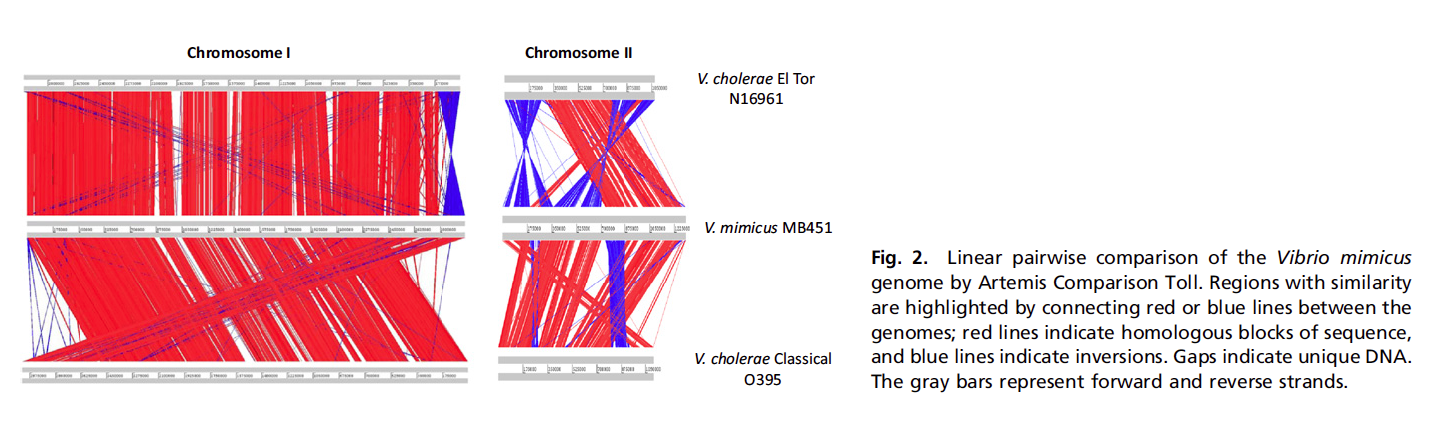
\includegraphics[width=1\textwidth]{images/v_mimicus}
  \end{center}    
  Suggests \textcolor{hutton_blue}{modularity of genome organisation, as a mechanism for adaptation} (HGT, two-speed genome).
\end{frame}

% SERRATIA SYMBIOTICA
\begin{frame}
  \frametitle{\textit{Serratia symbiotica} 
  \footnote{\tiny{\href{http://dx.doi.org/10.1093/gbe/evr002}{Burke and Moran (2011) \textit{Genome Biol. Evol.} \textbf{3}:195-208 doi:10.1093/gbe/evr002}}}
  }
  \textit{S. symbiotica} is a recently evolved symbiont of aphids\\
  \textcolor{hutton_green}{Massive genomic decay: consequence of adaptation}\\
  \begin{center}
    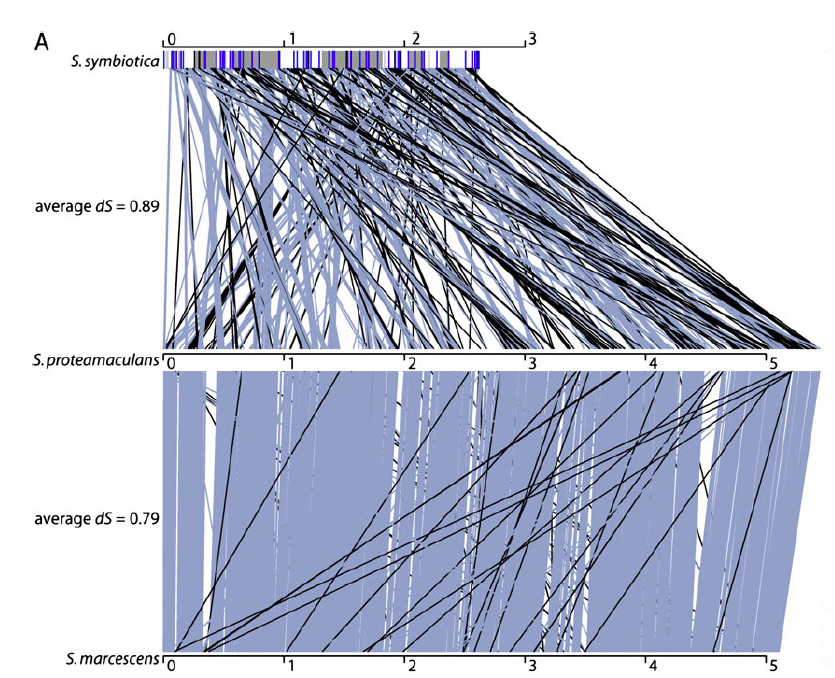
\includegraphics[width=0.75\textheight]{images/s_symbiotica}
  \end{center}    
\end{frame}


% WHOLE GENOME CLASSIFICATION
\begin{frame}
  \frametitle{Whole genome classification
  \footnote{\tiny{\href{http://dx.doi.org/10.1016/j.tim.2016.02.004}{Baltrus (2016) \textit{Trends Microbiol.} doi:10.1016/j.tim.2016.02.004}}}
    \footnote{\tiny{\href{http://dx.doi.org/10.1039/c5ay02550h}{Pritchard \textit{et al}. (2016) \textit{Anal. Methods} doi:10.1039/c5ay02550h}}}
  }
      \begin{itemize}  
        \item \textcolor{hutton_green}{Widespread confusion about strain classification and nomenclature}
          \begin{itemize}
            \item Taxonomies contradicted by bioinformatic classification
            \item Databases populated by non-taxonomists
          \end{itemize}
        \item \textcolor{hutton_blue}{Philosophy and practice of taxonomy are in conflict}
        \item \textcolor{hutton_purple}{Classification can be independent of existing nomenclature}
          \begin{itemize}
            \item The route from genotype to phenotype is complicated
            \item Time to abandon traditional microbial species concepts?
          \end{itemize}
          \item \textcolor{red}{An unambiguous sequence-based classification scheme is possible}
        \end{itemize}  
\end{frame}


% DNA-DNA HYBRIDISATION
\begin{frame}
  \frametitle{DNA-DNA hybridisation\footnote{\tiny{\href{http://dx.doi.org/10.1016/S0168-6445(00)00040-1}{Morello-Mora and Amann (2001) \textit{FEMS Micro. Rev.} doi:10.1016/S0168-6445(00)00040-1}}}}
  \begin{columns}[T]
    \begin{column}{5cm}
      \begin{itemize}
        \item ``Gold Standard'' for prokaryotic taxonomy, since 1960s. \textcolor{hutton_green}{``70\% identity $\approx$ same species.''}
        \item Denature DNA from two organisms.
        \item Allow to anneal. \textcolor{hutton_blue}{Reassociation $\approx$ similarity}, measured as $\Delta T$  of denaturation curves.
      \end{itemize}
    \end{column}
    \begin{column}{5cm}
      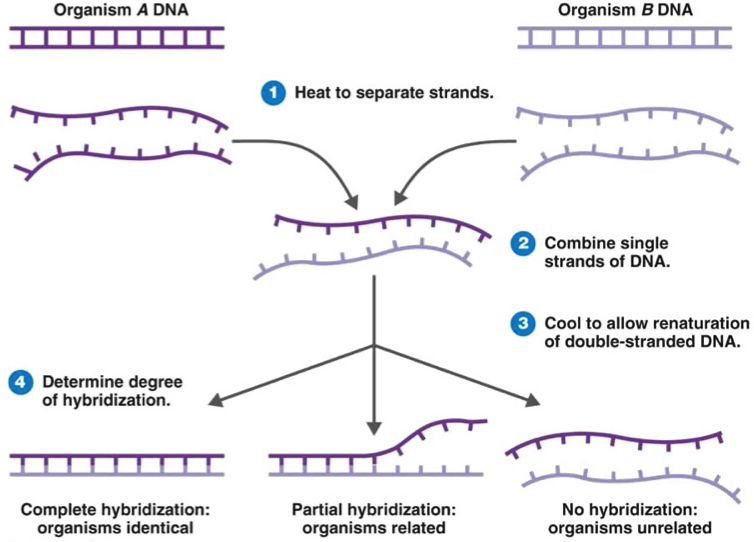
\includegraphics[width=1\textwidth]{images/dna-dna_hyb}
    \end{column}
  \end{columns}
\vspace{0.25cm}
\textcolor{hutton_purple}{Proxy for sequence similarity - replace with genome analysis\footnote{\tiny{\href{http://dx.doi.org/10.1186/1471-2180-12-302}{Chan \textit{et al} (2012) \textit{BMC Microbiol.} doi:10.1186/1471-2180-12-302}}}}?
\end{frame}

% ANIm
\begin{frame}
  \frametitle{Average Nucleotide Identity (ANIm)\footnote{\tiny{\href{http://dx.doi.org/10.1073/pnas.0906412106}{Richter and Rossello-Mora (2009) \textit{Proc. Natl. Acad. Sci. USA} doi:10.1073/pnas.0906412106}}}}
  \begin{columns}[T]
    \begin{column}{3cm}
      1. Align genomes (MUMmer)\\
      2. \textcolor{hutton_green}{\textbf{ANIm}: Mean \% identity of all matches} \\[0.25cm]
      \begin{itemize}
        \item DDH:ANIm linear
        \item \textcolor{hutton_blue}{70\%ID $\approx$ 95\%ANIb}
      \end{itemize}
    \end{column}
    \begin{column}{7cm}
      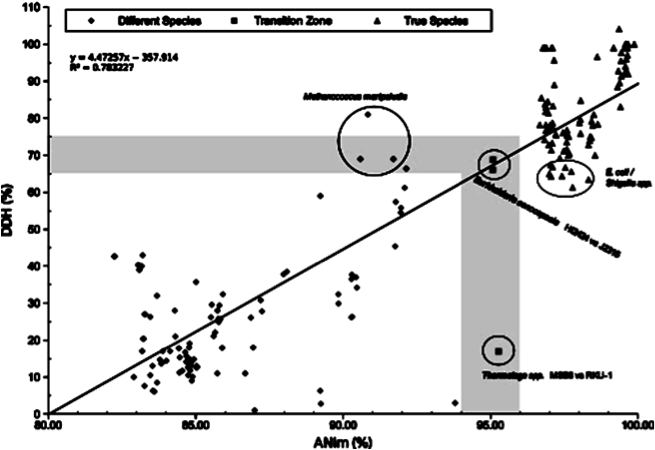
\includegraphics[width=1\textwidth]{images/ddh_anim}
    \end{column}
  \end{columns}
\end{frame}

% ANIm in practice
\begin{frame}
  \frametitle{55 Pectobacterium spp. ANIm
  \footnote{\tiny{\href{http://dx.doi.org/10.1039/c5ay02550h}{Pritchard \textit{et al}. (2016) \textit{Anal. Methods} doi:10.1039/c5ay02550h}}}
  }
  \begin{columns}[T]
    \begin{column}{3cm}
      \begin{itemize}
        \item Ten species-level groups (four novel)
        \item \small{\textit{P. carotovorum} split: several species}
        \item \small{\textit{P. wasabiae} split: two species}
      \end{itemize}
    \end{column}
    \begin{column}{7cm}
      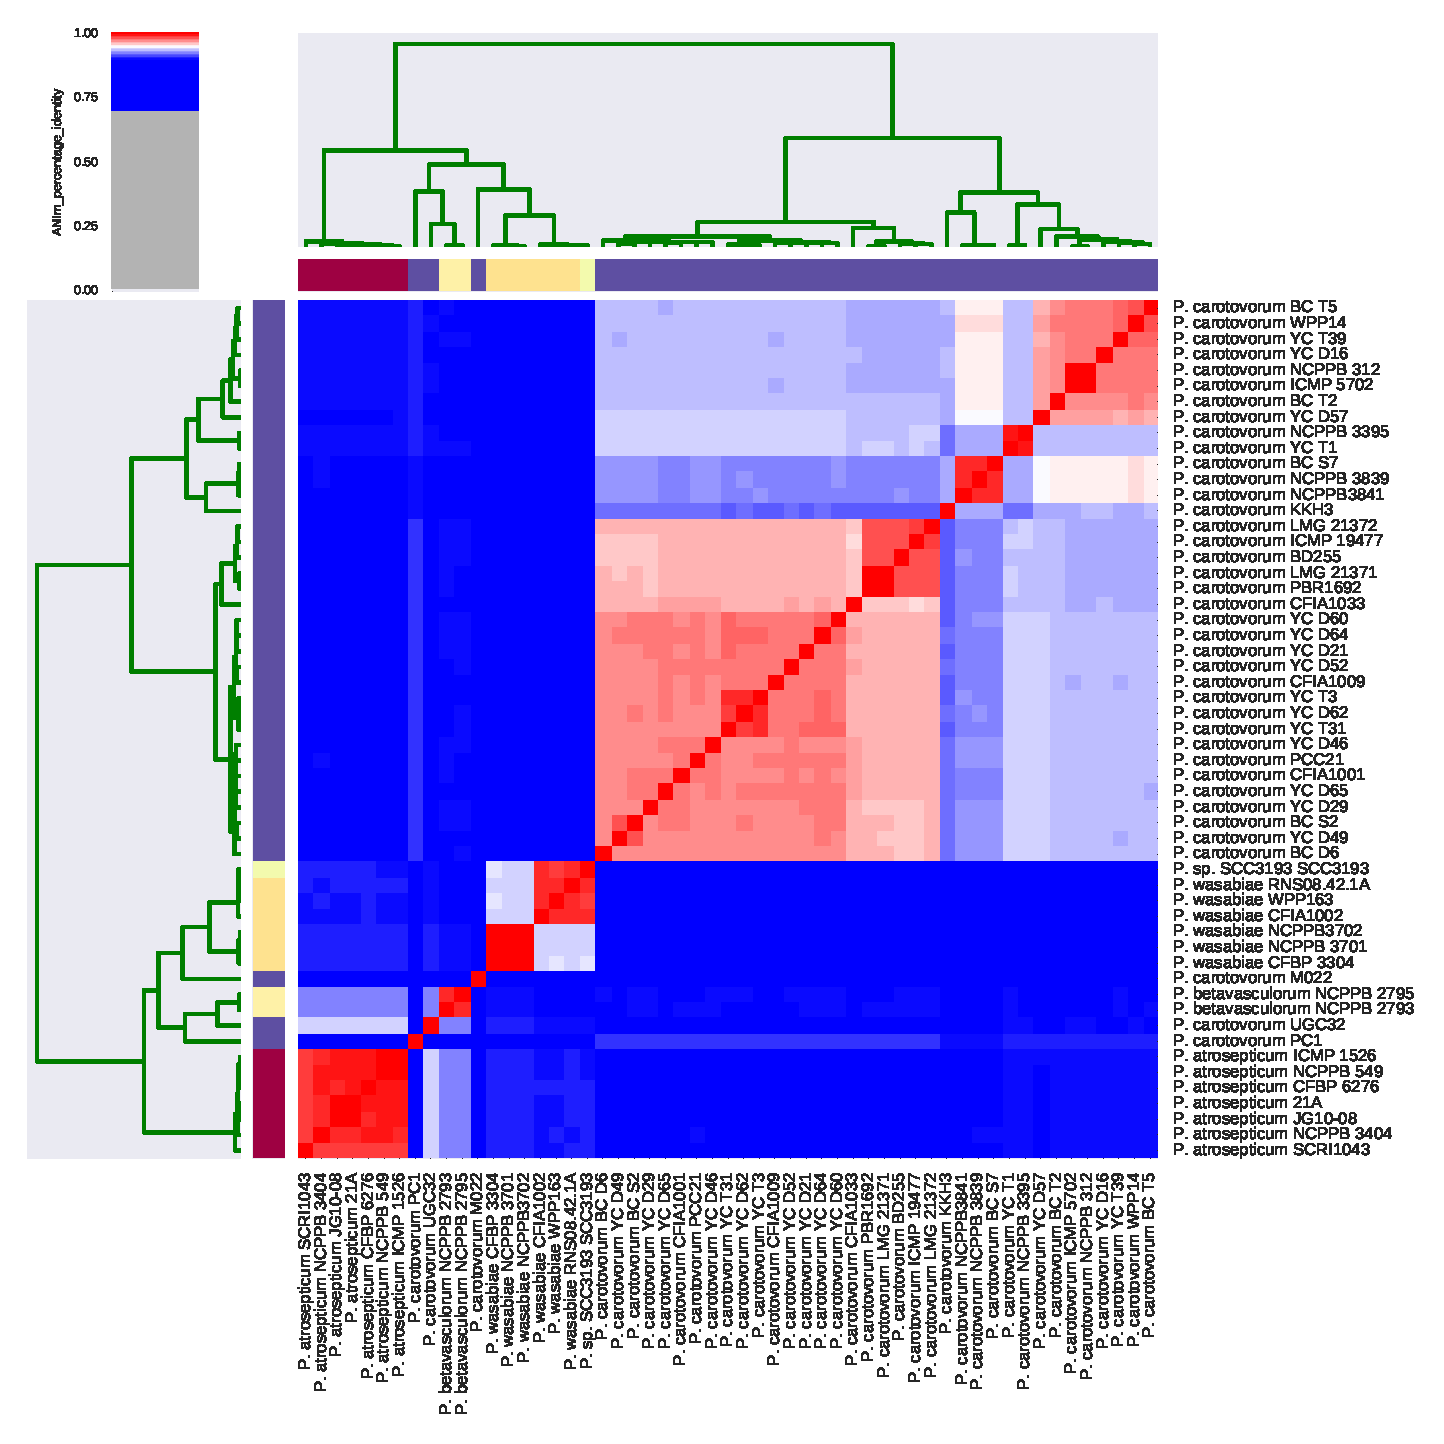
\includegraphics[width=1\textwidth]{images/Pectobacterium_ANIm_percentage_identity}
    \end{column}
  \end{columns}
\end{frame}

% ANIm in practice
\begin{frame}
  \frametitle{55 Pectobacterium spp. ANIm\footnote{\tiny{\href{http://dx.doi.org/10.1039/c5ay02550h}{Pritchard \textit{et al}. (2016) \textit{Anal. Methods} doi:10.1039/c5ay02550h}}}}
  \begin{columns}[T]
    \begin{column}{3cm}
      \begin{itemize}
        \item All isolates align over $>$50\% of whole genome
      \end{itemize}
    \end{column}
    \begin{column}{7cm}
      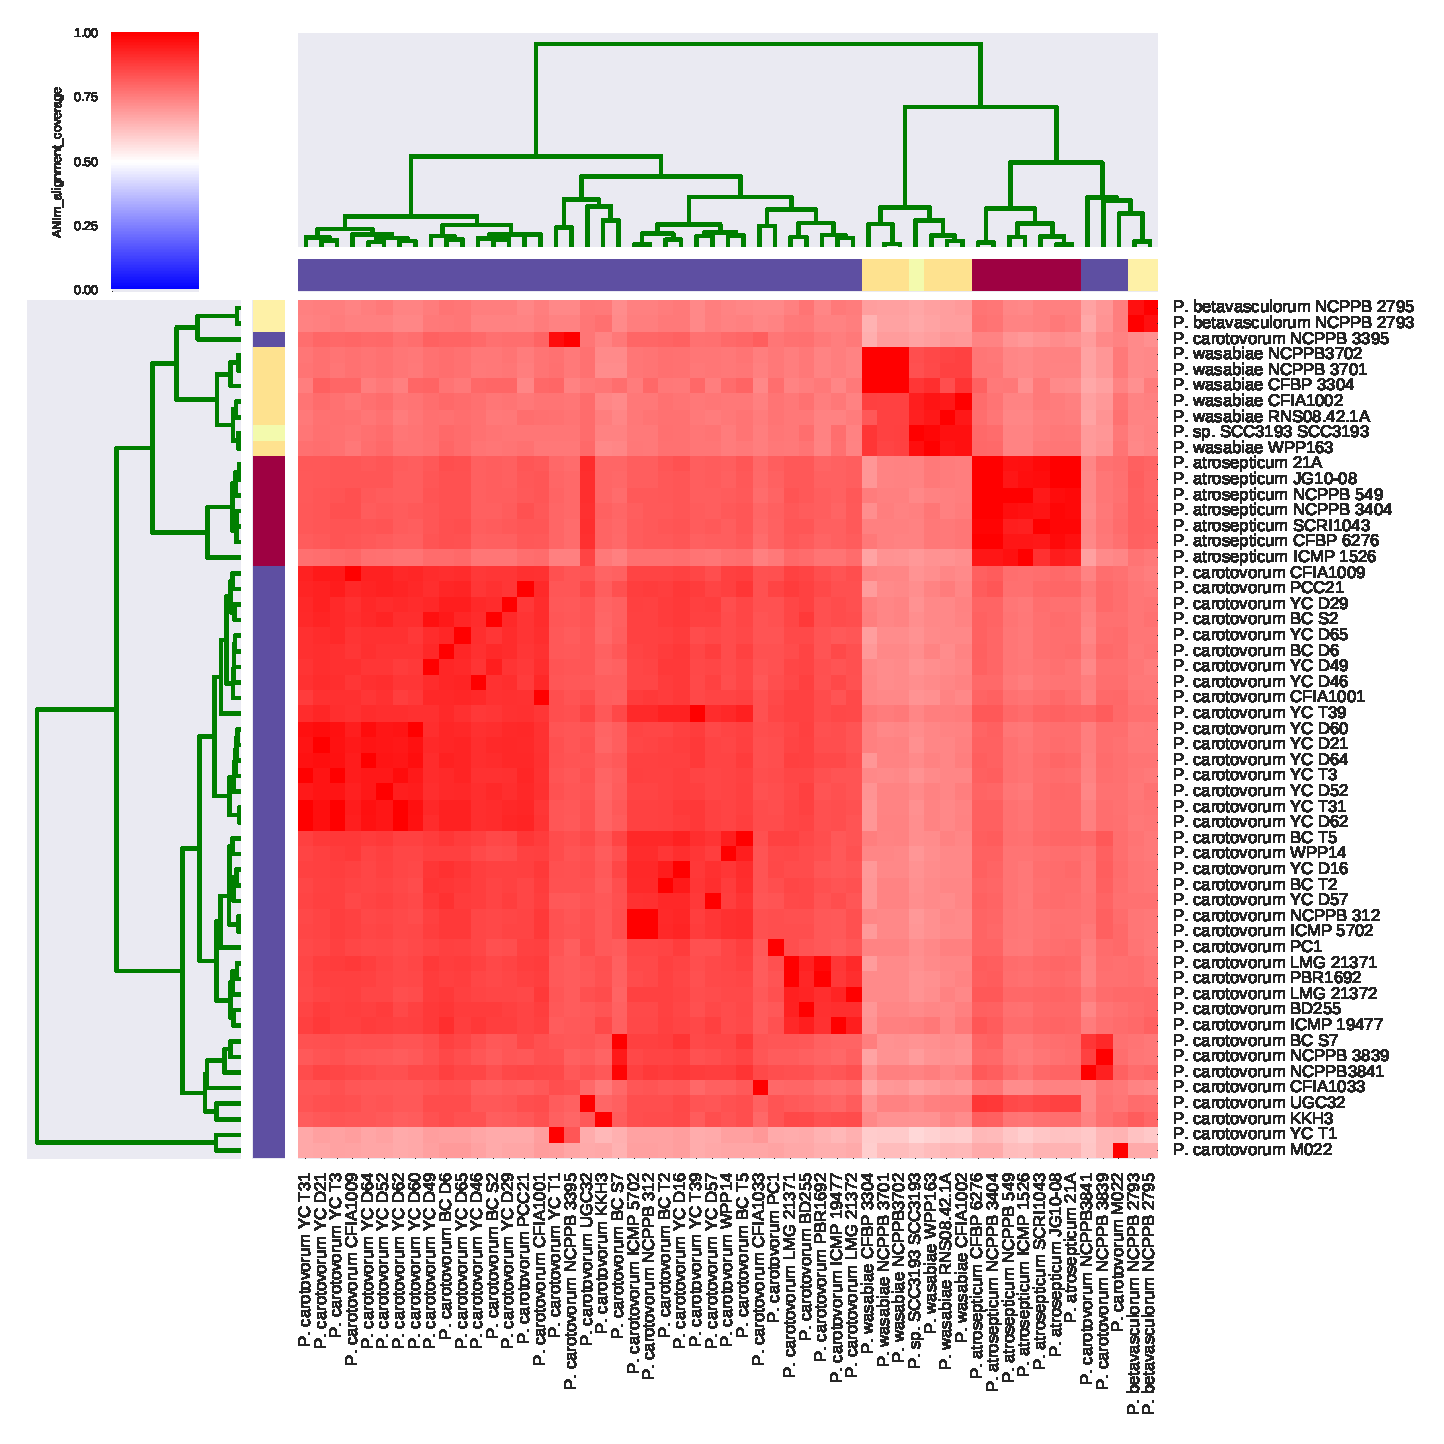
\includegraphics[width=1\textwidth]{images/Pecto_ANIm_alignment_coverage}
    \end{column}
  \end{columns}
\end{frame}

% ANI
\begin{frame}
  \frametitle{ANI}
  \begin{alertblock}{Advantages}
    \begin{itemize}
      \item Average identity of all `homologous' regions
      \item Approximates limiting case of MLST/MLSA/multigene comparisons
      \item Adaptable to variable thresholding (LINS) classifications
    \end{itemize}    
  \end{alertblock}
  \begin{block}{Criticisms}
    \begin{itemize}
      \item Thresholds `arbitrary', based on homologous regions only
      \item Taxonomic classification, not phylogenetic reconstruction
      \item No functional (or gene-based) interpretation; still need pangenome classification and analysis
    \end{itemize}
  \end{block}
\end{frame}

% EXERCISE
\begin{frame}
  \frametitle{EXERCISE}
  \begin{alertblock}{\url{exercises/01-whole_genome_comparisons.ipynb}}
    \begin{itemize}
      \item Pairwise comparison of \textit{Pseudomonas} genomes
      \item ANIm classification of \textit{Pseudomonas} isolates
    \end{itemize}
  \end{alertblock}
  \begin{itemize}
    \item \textcolor{hutton_purple}{\href{http://mybinder.org/repo/widdowquinn/Teaching-EMBL-Plant-Path-Genomics}{MyBinder link}}
  \end{itemize}
\end{frame}

% CHROMOSOME PAINTING
\begin{frame}
  \frametitle{Chromosome painting
  \footnote{\tiny{\href{http://dx.doi.org/10.1093/molbev/mst055}{Yahara \textit{et al}. (2013) \textit{Mol. Biol. Evol.} \textbf{30}:1454-1464 doi:10.1093/molbev/mst055}}}
  }
  \begin{itemize}
    \item ``Chromosome painting'' (\textcolor{hutton_purple}{\href{http://www.paintmychromosomes.com/}{FINESTRUCTURE}}) infers recombination-derived `chunks'\\
    \item Genome's haplotype constructed in terms of recombination events from a `donor' to a `recipient' genome\\
  \end{itemize}
  \begin{center}
    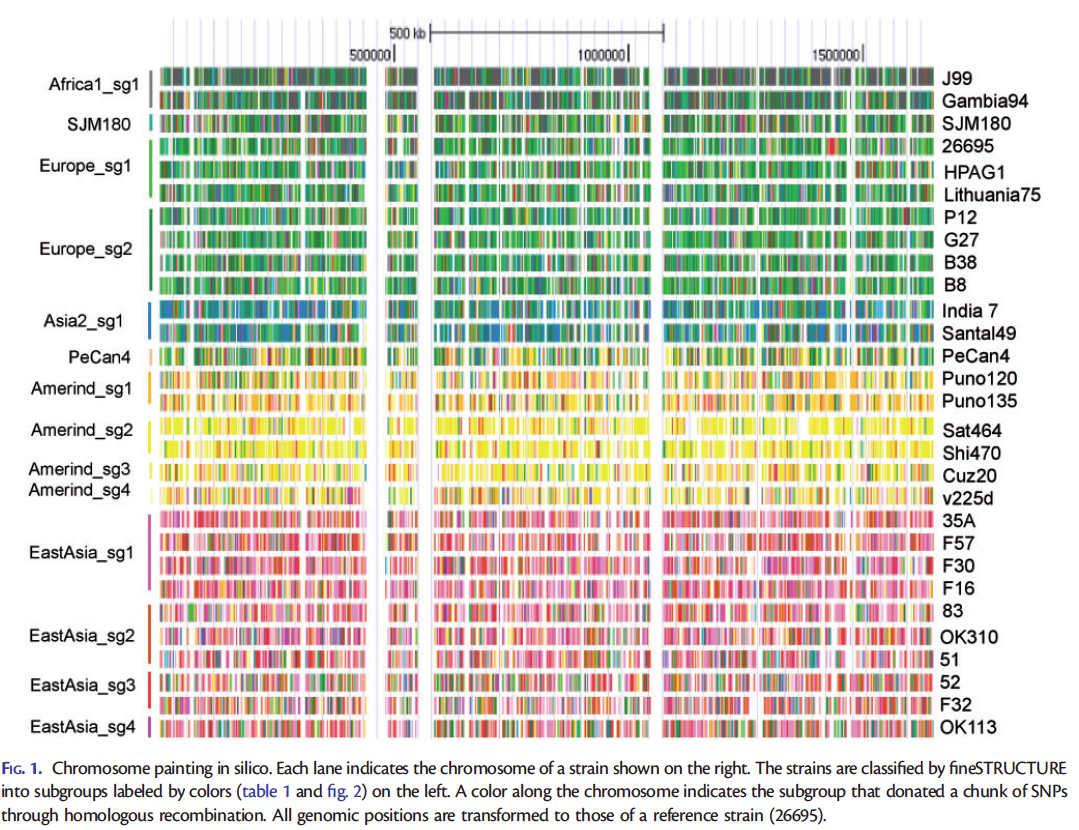
\includegraphics[width=0.6\textwidth]{images/chromosome_painting}
  \end{center}     
\end{frame}

% DNA-DNA hybridisation
\begin{frame}
  \frametitle{Chromosome painting
  \footnote{\tiny{\href{http://dx.doi.org/10.1093/molbev/mst055}{Yahara \textit{et al}. (2013) \textit{Mol. Biol. Evol.} \textbf{30}:1454-1464 doi:10.1093/molbev/mst055}}}
  }
  \begin{itemize}
    \item Recombination events summarised in a \textit{coancestry matrix}.\\
    \item \textit{H. pylori}: most within geographical bounds, but asymmetrical donation from Amerind/East Asian to European isolates.
  \end{itemize}
  \begin{center}
    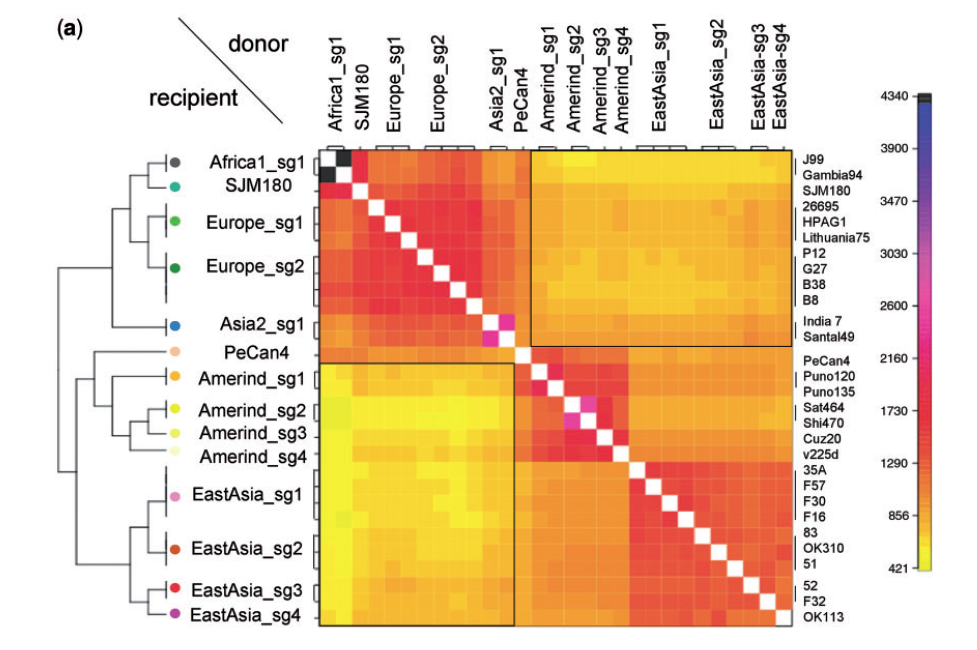
\includegraphics[width=0.75\textwidth]{images/coancestry}
  \end{center}     
\end{frame}


%% SUBSECTION
%% Levels of genome comparison (species, genus, etc.)
%\subsection{Levels of genome comparison}
%\input{sections/cladograms}
%\input{sections/ltee}
%\input{sections/neanderthal_2016}
%
%%%
% SECTION: Making Comparisons
%\section{Making Comparisons}
%% Types of genome comparison (whole genome, features, etc.)
%\input{sections/comparison_types}
% SUBSECTION
% Computational comparisons
%\subsection{In silico bulk genome comparisons}
%\input{sections/bulk_genome_comparisons}
% SUBSECTION
% Genome feature comparisons
%\subsection{Genome feature comparisons}
%\input{sections/genome_feature_comparisons}


%%%
% LICENCE FOR REUSE
%% licence.tex
%% Author: Leighton Pritchard
%% Copyright: James Hutton Institute
%% These slides describe the licence for reuse of these slides and
%% materials

%
\begin{frame}
  \frametitle{Licence: CC-BY-SA}
  By: Leighton Pritchard \\[0.5cm]
  This presentation is licensed under the Creative Commons Attribution ShareAlike license \\
  \href{https://creativecommons.org/licenses/by-sa/4.0/}{https://creativecommons.org/licenses/by-sa/4.0/}
\end{frame}

% etc
\end{document}